\subsection{Gebrochen rationale Funktionen}

\[
    y = f(x) = \frac{a_0 + a_1 x^1 + a_2 x^2 + \cdots + a_z x^z}
    {b_0 + b_1 x^1 + b_2 x^2 + \cdots + b_z x^n}
    = \frac{\sum_{i=0}^{z} a_i\ x^i}{\sum_{i=0}^{n} b_i\ x^i}
\]

für \(n > 0\) und \(z < n\): echt gebrochen

für \(n > 0\) und \(z \geq n\): unecht gebrochen

\paragraph{Unecht gebrochene Funktionen}

\[
    G(x) = \frac{Z(x)}{N(x)} = \underbrace{S(x)}_{\text{ganze Fkt.}} + \underbrace{\frac{R(x)}{N(x)}}_{\text{echt gebrochen}}
\]

\subsubsection{Beispiele}

\paragraph{1. Beispiel (einfachste gebrochene Funktion) (siehe Abb.~\ref{fig:gebrochenefunktionen_beispiel1})}

\[
    y = f(x) = \frac{1}{x}  
\]

punktsymmetrisch

\begin{figure}[H]
    \centering
    \begin{tikzpicture}
        \begin{axis}[
            default,
            xmin=-4.2, xmax=4.2,
            ymin=-4.2, ymax=4.2,
            width=6cm
            ]
            \draw [orange, smooth, samples=100, domain=-4:-1/100] plot (\x, {1 / \x});
            \draw [orange, smooth, samples=100, domain=1/100:4] plot (\x, {1 / \x});
        \end{axis}
    \end{tikzpicture}
    \caption{\(f(x) = \frac{1}{x}\)}\label{fig:gebrochenefunktionen_beispiel1}
\end{figure}

\paragraph{2. Beispiel  (siehe Abb.~\ref{fig:gebrochenefunktionen_beispiel2})}

\[
    y = f(x) = \frac{1}{x^2}  
\]

achsensymmetrisch

\begin{figure}[H]
    \centering
    \begin{tikzpicture}
        \begin{axis}[
            default,
            xmin=-4.2, xmax=4.2,
            ymin=-4.2, ymax=4.2,
            width=6cm
            ]
            \draw [orange, smooth, samples=100, domain=-4:-1/10] plot (\x, {1 /
            (pow(\x, 2))});
            \draw [orange, smooth, samples=100, domain=1/10:4] plot (\x, {1 /
            (pow(\x, 2))});
        \end{axis}
    \end{tikzpicture}
    \caption{\(f(x) = \frac{1}{x^2}\)}\label{fig:gebrochenefunktionen_beispiel2}
\end{figure}

\paragraph{2. Beispiel verschoben}

\[
    y = f(x) = \frac{1}{{(x-1)}^2}  
\]

\begin{figure}[H]
    \centering
    \begin{tikzpicture}
        \begin{axis}[
            default,
            xmin=-4.2, xmax=4.2,
            ymin=-4.2, ymax=4.2,
            width=6cm
            ]
            \draw [orange, smooth, samples=100, domain=-4:9/10] plot (\x, {1 /
            (pow((\x - 1), 2))});
            \draw [orange, smooth, samples=100, domain=11/10:4] plot (\x, {1 /
            (pow((\x - 1), 2))});
            \draw[dashed, gray] (1, -4) -- (1, 4);
        \end{axis}
    \end{tikzpicture}
    \caption{\(f(x) = \frac{1}{{(x-1)}^2}\)}\label{fig:gebrochenefunktionen_beispiel3}
\end{figure}

\subsubsection{Umgang mit gebrochenen Funktionen}

\begin{figure}[H]
    \centering
    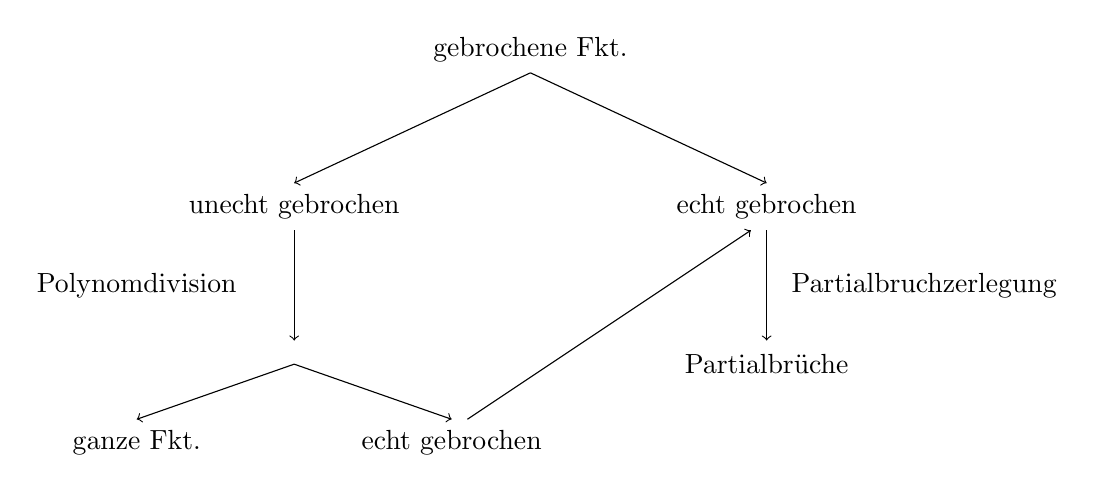
\begin{tikzpicture}
        \node[] at (0, 1) {gebrochene Fkt.};
        \node[] at (-3,-1) {unecht gebrochen};
        \node[] at (3,-1) {echt gebrochen};
        \node[] at (-5, -2) {Polynomdivision};
        \node[] at (-5, -4) {ganze Fkt.};
        \node[] at (-1, -4) {echt gebrochen};
        \node[] at (5, -2) {Partialbruchzerlegung}; 
        \node[] at (3, -3) {Partialbrüche}; 

        \draw[->] ( 0, 0.7) -- (-3,-0.7);
        \draw[->] ( 0, 0.7) -- ( 3,-0.7);
        \draw[->] (-3, -1.3) -- (-3,-2.7);
        \draw[->] (-3, -3)   -- (-5,-3.7);
        \draw[->] (-3, -3)   -- (-1,-3.7);
        
        \draw[->] (-0.8, -3.7) -- (2.8, -1.3);
        
        \draw[->] (3, -1.3) -- (3, -2.7);
    \end{tikzpicture}
    \caption{Umgang mit gebrochenen Funktionen}\label{fig:gebrochene_funktionen_graph}
\end{figure}

\subsubsection{Partialbruchzerlegung}

\[
    y = \frac{5x + 11}{x^2 + 3x - 10}    
\]

\paragraph{I.\;Prüfen: Wirklich echt gebrochen?}

\textit{Ja}

\paragraph{II.\;Nullstellen des Nenners}

\begin{gather*}
    x^2 + 3x - 10 = 0 \\
    x_{1,2} = -\frac{3}{2} \pm \sqrt{\frac{9}{4}+ \frac{40}{4}} = -\frac{3}{2} \pm \frac{7}{2} \\
    x_1 = 2 \quad x_2 = -5
\end{gather*}

\[
    \Rightarrow \frac{5x + 11}{(x-2)(x + 5)}
\]

\paragraph{III.\;Aufstellen der Partialbrüche}

\begin{align*}
    \frac{5x + 11}{(x-2)(x + 5)} &= \frac{A}{x - 2} + \frac{B}{x + 5} &&\mid \cdot ((x-2)(x+5)) \\
    5x + 11 &= A(x + 5) + B(x - 2)
\end{align*}

\paragraph{IV.\;Konstanten bestimmen}

Durch Einsetzen von Werten (Optimalerweise den Nullstellen):

\begin{align*}
    5x + 11 &= A(x + 5) + B(x - 2) \\
    \\
    x = 2:\\
    21 &= 7A  \Leftrightarrow A = \frac{21}{7} = 3 \\
    x = -5:\\
    -14 &= -7B \Leftrightarrow B = 2
\end{align*}

\paragraph{V.\;Einsetzen}

\[
    y = \frac{5x + 11}{x^2 + 3x - 10} = \frac{3}{x-2} + \frac{2}{x+5}  
\]

\paragraph{Anmerkung}

Die Partialbruchzerlegung ist ein Lösungsverfahren für Integrale, ist normalerweise nicht von Vorteil für
die Kurvendiskussion:

\[
    \int \frac{5x + 11}{x^2 + 3x - 10} \diff x = \int \frac{3}{x-2} \diff x + \int \frac{2}{x+5} \diff x 
\]

\paragraph{Fallunterscheidung}

\subparagraph{1. Fall}

\(N(x)\) hat nur einfache reelle Nullstellen, \(x_i\) sei eine dieser
Nullstellen.

Dann gehört zu \(x_i\) ein Partialbruch der Form:

\[
    \frac{A_i}{x - x_i}    
\]

\subparagraph{2. Fall}

\(N(x)\) hat an der Stelle \(x_i\) eine \(k\)-fache Nullstelle.

Dann gehören zu \(x_i\) \(k\) Partialbrüche der Form:

\[
    \frac{A_{i1}}{x - x_i}  + \frac{A_{i2}}{{(x - x_i)}^2} + \frac{A_{i3}}{{(x - x_i)}^3} + \cdots + \frac{A_{ik}}{{(x - x_i)}^k}   
\]

\subsubsection{Polynomdivision}

\[
	f(x) = x^3 + x^2 -8x - 12
\]

geschätzte Nullstelle: \(x_1 = 3\) \textrightarrow\ Polynomdivision:
\footnote{Aus technischen Gründen ist die Polynomdivision hier mit bereits aufgelösten Minusklammern dargestellt.}

\polyset{style=C, div=:,vars=x}
\polylongdiv{x^3 + x^2 -8x -12}{x -3}

\begin{uebung}
	Diskutieren Sie ohne Ableitung.

	\begin{question}
		\[
			y = \frac{x^3}{{(x-1)}^2}
		\]
	\end{question}

	\begin{solution}
		\[
			y = \frac{x^3}{{(x-1)}^2}
		\]

		\subparagraph{Nullstellen}
		Dreifache Nullstelle bei \(x = 0 \Rightarrow \) Sattelpunkt

		\subparagraph{Polstelle}
		Zweifache Polstelle bei \(x = 1 \Rightarrow \) PS ohne Vorzeichenwechsel

		\subparagraph{Symmetrie}
		weder gerade noch ungerade: nicht symmetrisch

		\subparagraph{Polynomdivision}
		\polyset{style=C, div=:,vars=x}
		\polylongdiv{x^3}{x^2 -2x + 1}

		\[
			y = \underbrace{x + 2}_{\text{\color{cyan}Asymptote}} + \underbrace{\frac{3x - 2}{{(x - 1)}^2}}_{\text{echt gebrochen}}
		\]

		\begin{figure}[H]
			\centering
			\begin{tikzpicture}
				\begin{axis}[
						default,
						xmin=-8.2, xmax=8.2,
						ymin=-8.2, ymax=8.2,
						width=8cm
					]
					\draw [color1, smooth, samples=100, domain=-8.2:0.9] plot (\x, {pow(\x, 3) / pow((\x - 1), 2)});
					\draw [color1, smooth, samples=100, domain=1.1:8.2] plot (\x, {pow(\x, 3) / pow((\x - 1), 2)});
					\draw [dashed, cyan, samples=100, domain=-8.2:8.2] plot (\x, {\x+2});
					\draw[dashed, gray] (1, -8.2) -- (1, 8.2);
				\end{axis}
			\end{tikzpicture}
			\caption{Skizze}
		\end{figure}
	\end{solution}

	\begin{question}
		\[
			y = x^3 + x^2 - 8x - 12
		\]
	\end{question}

	\begin{solution}
		\[
			y = x^3 + x^2 - 8x - 12
		\]

		\subparagraph{Nullstellen}
		1. Nullstelle raten: \(x_{N1} = 3\)

		\polyset{style=C, div=:,vars=x}
		\polylongdiv{x^3 + x^2 -8x -12}{x -3}

		2./3. Nullstelle bei \(x_{N2} = -2 \Rightarrow \) Extremwert (2-fache Nullstelle)

		\subparagraph{Symmetrie}
		weder gerade noch ungerade: nicht symmetrisch

		\[
			\limtoinfty{x} y = \infty; \limtomininfty{x} y = -\infty
		\]

		\begin{figure}[H]
			\centering
			\begin{tikzpicture}
				\begin{axis}[
						xmin=-8.2, xmax=8.2,
						ymin=-8.2, ymax=8.2,
						height=8cm,
						width=8cm,
						grid=both,
						axis lines=middle,
						grid style={line width=.1pt, draw=gray!20},
						major grid style={line width=.2pt,draw=gray!50},
						ticklabel style={font=\tiny},
						xlabel style={font=\tiny},
						ylabel style={font=\tiny},
						xlabel={x}, ylabel={y}
					]
					\draw [color1, smooth, samples=100, domain=-4:4] plot
					(\x, {pow(\x, 3) + pow(\x,2) - 8 * \x - 12});
				\end{axis}
			\end{tikzpicture}
			\caption{Skizze}
		\end{figure}
	\end{solution}
\end{uebung}

